% asset_id: FAS1ComplexNumbersLociRegionsTikZ-001
\documentclass[tikz,border=8pt]{standalone}
\usepackage{amsmath}
\usepackage{xcolor}
\definecolor{Canvas}{HTML}{FAF9F6}
\definecolor{Ivory}{HTML}{FFFFF0}
\definecolor{SoftLine}{HTML}{E5E5EA}
\definecolor{TextInk}{HTML}{2C2C2E}
\definecolor{Gold}{HTML}{C5A059}
\definecolor{BrightGold}{HTML}{D4AF37}
\begin{document}
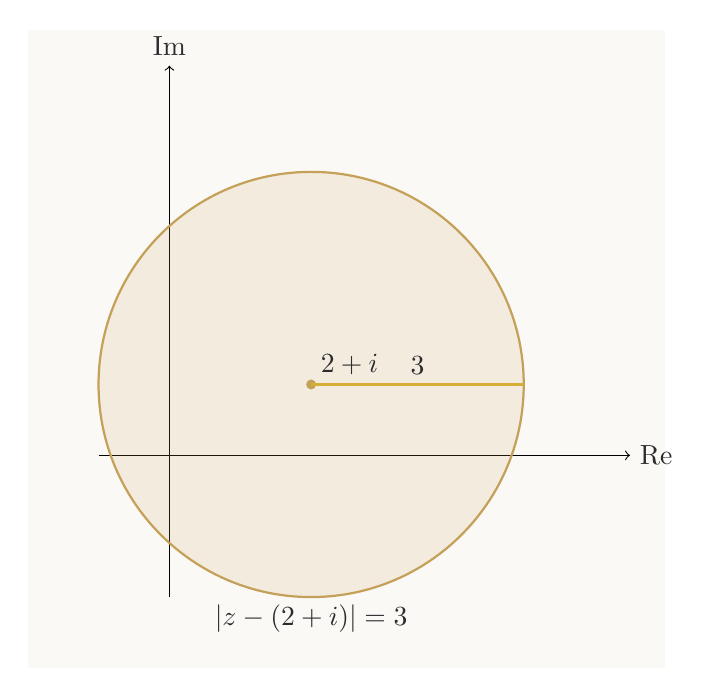
\begin{tikzpicture}[scale=0.9,every node/.style={text=TextInk}]
\fill[Canvas] (-2,-3) rectangle (7,6);
\draw[->] (-1,0)--(6.5,0) node[right] {$\operatorname{Re}$};
\draw[->] (0,-2)--(0,5.5) node[above] {$\operatorname{Im}$};
\fill[Gold,opacity=.15] (2,1) circle (3);
\draw[Gold,thick] (2,1) circle (3);
\fill[Gold] (2,1) circle (2pt) node[above right] {$2+i$};
\draw[BrightGold,thick] (2,1)--(5,1) node[midway,above] {$3$};
\node at (2,-2.3) {$\lvert z-(2+i)\rvert=3$};
\end{tikzpicture}
\end{document}
